\documentclass{standalone}
\usepackage{tikz}
\usetikzlibrary{patterns, angles}

\begin{document}
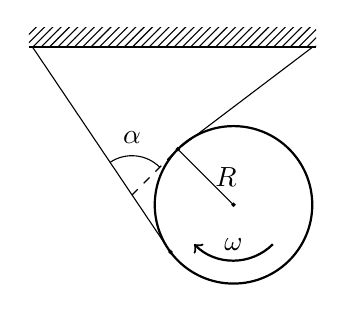
\begin{tikzpicture}
	\coordinate (A) at (-2.55,2);
	\coordinate (B) at (-1.29, 1.414-1.29);
	\coordinate (C) at (-0.707,0.707);

	\draw [thick] (0,0) circle (1);
	\draw [draw=none, pattern=north east lines] (-2.6,2) rectangle (1.05,2.25);
	\draw [thick] (-2.6,2) -- (1.05,2);
	\draw (C) -- (1,2);
	\draw (C) -- (0,0) node [midway, right=0pt] {$R$};
	\draw [fill] (0,0) circle (0.02);
	\draw [fill] (C) circle (0.02);
	\draw [fill] (-0.8,-0.6) circle (0.02);
	\draw (-0.8,-0.6) -- (A);
	\draw [thick, ->] (0.5, -0.5) arc (-45:-135:0.707) node [above,midway] {$\omega$};	
	\pic [draw, -, angle eccentricity=1.5] {angle = C--B--A};
	\node [above=15pt] at (B) {$\alpha$};
	\draw [dashed] (B) -- (C);
\end{tikzpicture}
\end{document}